\documentclass[11pt]{article}

\usepackage[margin=0.78in, top=0.82in, bottom=0.86in]{geometry}
\usepackage{times}
\usepackage{amsmath,amssymb}
\usepackage{graphicx}
\usepackage{hyperref}
\usepackage{natbib}
\usepackage{booktabs}
\usepackage{enumitem}
\usepackage{xcolor}
\usepackage[T1]{fontenc}
\usepackage{setspace}
\usepackage{titlesec}
\usepackage{tikz}
\usepackage{pgfplots}
\usepackage{pgfplotstable}
\usepackage{subcaption}
\usepackage{placeins}

\usetikzlibrary{arrows.meta, positioning, shapes.geometric, calc, fit}
\usepgfplotslibrary{groupplots}
\pgfplotsset{compat=1.18}

\setstretch{0.94}
\setlength{\parskip}{0.28em}
\setlength{\parindent}{0pt}
\titlespacing*{\section}{0pt}{0.75em}{0.32em}
\titlespacing*{\subsection}{0pt}{0.58em}{0.25em}
\titlespacing*{\subsubsection}{0pt}{0.45em}{0.18em}
\makeatletter
\setlength{\@fptop}{0pt}
\setlength{\@fpsep}{12pt}
\setlength{\@fpbot}{0pt plus 1fil}
\makeatother

\hypersetup{colorlinks=true, linkcolor=blue, citecolor=blue, urlcolor=blue}

\newcommand{\FinalRunId}{0be5c8d2a37943949e33ae431bf63bd0}
\newcommand{\FinalNumPrompts}{200}
\newcommand{\PagAvgNfe}{72.070}
\newcommand{\AdaAvgNfe}{90.800}
\newcommand{\AvgNfeDelta}{-18.730}
\newcommand{\MedNfeDelta}{-18.000}
\newcommand{\AvgNfeRatio}{0.786}
\newcommand{\PagAccPct}{89.500}
\newcommand{\AdaAccPct}{89.500}
\newcommand{\PagCorrect}{179}
\newcommand{\AdaCorrect}{179}
\newcommand{\AvgRuntimeDelta}{-0.050}
\newcommand{\MedRuntimeDelta}{0.005}
\newcommand{\NfeWinCount}{199}
\newcommand{\NfeTieCount}{0}
\newcommand{\NfeLossCount}{1}
\newcommand{\PagAvgBlocks}{15.460}
\newcommand{\AdaAvgBlocks}{15.660}
\newcommand{\SchedulerAvgMs}{64.076}
\newcommand{\BestSavingPrompt}{gsm8k\_test\_0370}
\newcommand{\BestSavingDelta}{-51}
\newcommand{\WorstOverheadPrompt}{gsm8k\_test\_0374}
\newcommand{\WorstOverheadDelta}{1}
\newcommand{\PagBlockRows}{3092}


\newcommand{\projectname}{Phase-Adaptive Generation}
\newcommand{\pag}{PAG}
\newcommand{\dllm}{dLLM}
\newcommand{\nfe}{NFE}
\newcommand{\code}[1]{\texttt{#1}}

\tikzset{
  stage/.style={draw, rounded corners=2pt, align=center, minimum height=0.72cm,
    minimum width=2.15cm, fill=blue!7, font=\small},
  data/.style={draw, rounded corners=2pt, align=center, minimum height=0.62cm,
    minimum width=2.0cm, fill=orange!10, font=\small},
  modelbox/.style={draw, rounded corners=2pt, align=center, minimum height=0.72cm,
    minimum width=2.25cm, fill=green!8, font=\small},
  arrow/.style={-{Latex[length=2mm]}, thick}
}

\begin{document}

\begin{center}
{\LARGE\bfseries Phase-Adaptive Generation: Learned Compute Scheduling for Diffusion Language Models}\\[0.35em]
{\large Keshav Krishna \quad Prajesh Kumar \quad Siva Satvik Mandapati}\\[0.16em]
{\normalsize New York University, Building LLM Reasoners --- Spring 2026}\\
{\normalsize \texttt{\{kk6081, pg2973, sm12779\}@nyu.edu}}
\end{center}

\begin{abstract}
Diffusion language models decode by iteratively refining masked tokens, which exposes a useful scheduling question: should every part of a reasoning answer receive the same block size and refinement budget? We study this question through \projectname{} (\pag{}), a system for predicting block-level control tuples from generation traces and using them to adapt LLaDA decoding. The project produced three connected contributions. 
First, we built trace-analysis tooling for Dream and LLaDA, including token-level stabilization features, PELT/kernel change-point detection, and a Streamlit inspection interface. 
Second, we converted AdaBlock-style LLaDA traces into block-native training data and compared several next-control predictors, including a regression Transformer, a variable-order Markov baseline, a multi-output random forest, and a classification/ordinal Transformer over rich block features. 
Third, we integrated the learned predictor into a tuple-conditioned LLaDA scheduler and evaluated it against AdaBlock on 200 held-out GSM8K prompts. 
On the final run, PAG matched AdaBlock answer accuracy at \(89.5\%\) while reducing average total \nfe{} from \AdaAvgNfe{} to \PagAvgNfe{} per prompt, a \(\approx 21.4\%\) reduction, with a small predictor overhead of \(\SchedulerAvgMs\) ms per prompt. 
PAG also gave significant response time savings over vanilla AdaBlock with average runtime delta of PAG - AdaBlock being approximately 0.10 sec.
\end{abstract}

\section{Introduction}

Autoregressive language models spend one decoding step per output token. Diffusion language models (\dllm{}s) such as Dream and LLaDA instead produce text through iterative masked-token refinement, so they can commit multiple positions in a block. This creates an explicit compute-allocation problem. Some spans of a solution are syntactically predictable or copied from context; other spans contain arithmetic, variable binding, or answer-finalization steps. A fixed schedule treats both regimes similarly.

\pag{} asks whether generation traces contain enough phase structure to forecast the next block-level control decision. Our final control tuple is
\[
  y_t = (\text{block\_size}_t,\ \text{refinement\_budget}_t),
\]
where block size controls how many tokens are attempted together and refinement budget controls the number of model forward evaluations allowed before committing the block. The broader implementation supports richer conditioning fields: observed \nfe{}, stabilization/refinement steps, confidence statistics, digit fraction, delimiter fraction, and gap statistics.

The project evolved in two phases. We first treated phase discovery as an interpretability problem over token-level traces: collect Dream/LLaDA refinement histories, extract stabilization features, and segment them with change-point detection (CPD). This showed interpretable difficulty shifts but also exposed a label-construction problem: CPD boundaries move with the feature, smoothing window, and penalty. We therefore shifted to a block-native path based on AdaBlock traces, where block boundaries and compute budgets are directly observed. CPD remains useful for analysis, while training and scheduling use block-level tuples.

\section{Related Work}

\textbf{Diffusion language models.} Dream and LLaDA demonstrate that diffusion-style language generation can support reasoning, planning, and instruction following without left-to-right token generation~\citep{ye2025dream,nie2025llada}. Block Diffusion formalizes semi-autoregressive diffusion decoding as an interpolation between fully autoregressive and fully parallel generation~\citep{arriola2025block}. DiffuLLaMA and related adaptation work show that diffusion LMs can inherit strong language-model priors from autoregressive models~\citep{gong2025diffullama}.

\textbf{Efficient \dllm{} inference.} Fast-dLLM studies KV caching and parallel decoding for training-free acceleration~\citep{wu2025fastdllm}. AdaBlock-dLLM is the closest prior system to our final implementation: it adapts block length using confidence and semantic boundary heuristics~\citep{lu2025adablock}. Our contribution is complementary. Instead of only reacting to the current confidence band, we train predictors over realized block histories and feed their next-control predictions into the decoding loop.

\textbf{Sequence modeling and change-point detection.} Our predictor variants use compact Transformer encoders with sinusoidal positional encodings~\citep{vaswani2017attention}. Our early analysis used PELT-style CPD, which optimizes a penalized segmentation objective and prunes dynamic-programming states for efficiency~\citep{killick2012optimal}. In this project, CPD is an analysis and data-understanding tool rather than the final source of scheduler labels.

\section{System Overview}

PAG comprises two subsystems: an offline predictor-training pipeline that extracts block-level control tuples from AdaBlock LLaDA generation traces and trains a Transformer-based next-tuple predictor, and an online scheduler that loads the trained checkpoint and governs per-block refinement with a learned budget and soft-cap early exit.
Figure~\ref{fig:architecture} shows this overview.

\textbf{Predictor training.} We run AdaBlock-dLLM with LLaDA-8B-Instruct on 5{,}000 GSM8K training problems, recording one control tuple per decoded block. 
Each tuple captures the realized block size, the number of model forward evaluations (NFE), the mean and minimum top-1 softmax confidence across unmasked positions, the fraction of digit tokens in the block, and the fraction of delimiter tokens. 
The resulting corpus contains 138{,}901 tuples. For training, we construct sliding-window sequences of length eight: each window of past tuples predicts the next (\textit{block\_size}, \textit{refinement\_budget}) pair. 
Features are z-score normalized per field using corpus statistics. The predictor is a Transformer encoder (ablations over layers, heads, learning rate, pre-norm) with two output heads: a softmax classifier over 128 block-size classes and an ordinal regression head over 83 binary refinement-budget thresholds. 
The budget head receives the block-size logits as conditioning, allowing the model to capture that larger blocks often need different budgets. 
Training uses cross-entropy for block size and binary cross-entropy for ordinal thresholds with an AdamW optimizer and early stopping. 
The final checkpoint bundles model weights, normalization statistics, and the ordered feature-field list.

\textbf{Online scheduling.} At decode time, the checkpoint is loaded by a scheduler that maintains a rolling context of realized tuples. 
The first block completely simulates AdaBlock to get block coundary and refinement; subsequent blocks pad the observed history to the window length, forward it through the predictor, and clamp the output by remaining sequence length and configured minimum and maximum bounds. 
Block sizing follows AdaBlock's adaptive mechanism: the model identifies the highest-confidence delimiter token in a forward-looking window and positions the block boundary there, defaulting to a system-chosen length when no delimiter meets the threshold. 
The predictor supplies the refinement budget independently. Decoding proceeds as a threshold-based unmasking loop within the active block. Once the forward-evaluation count reaches the predicted budget, a soft-cap mechanism checks per-token confidence and stability: 
if the minimum unmasking confidence exceeds \(\tau_{\text{commit}} = 0.8\) or predictions have been stable for \(\tau_{\text{stable}} = 2\) steps, the block exits early or
when only a small fraction of the block remains and confidence is adequate, a forced commit terminates refinement unconditionally. 
After each block, the realized tuple---actual NFE, mean and minimum confidence, digit fraction, and delimiter fraction---is appended to the rolling context. 
The scheduler is a drop-in replacement within AdaBlock-dLLM's LLaDA generation harness, enabling per-prompt comparison against an unmodified AdaBlock run from the same random seed.

\begin{figure}[t!]
  \centering
  \resizebox{0.96\linewidth}{!}{%
    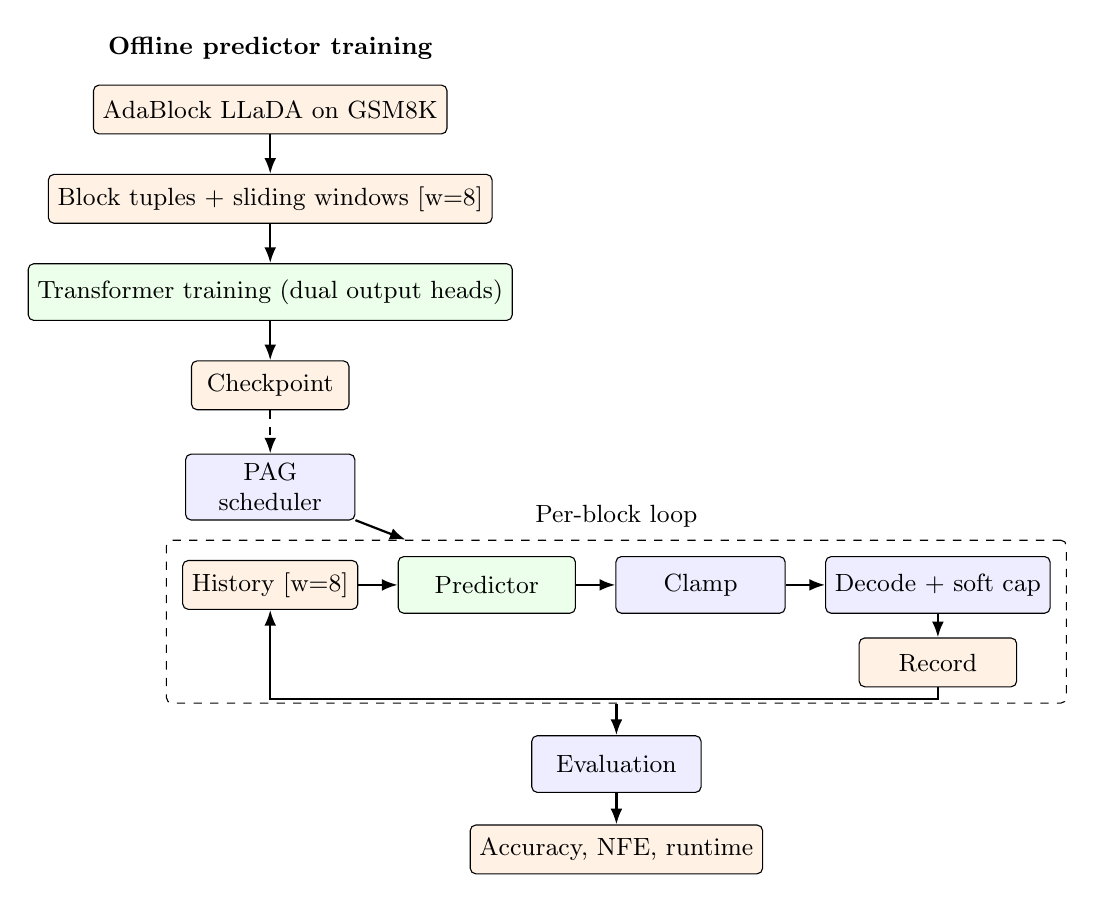
\begin{tikzpicture}[node distance=0.55cm and 0.5cm]
      % === Offline training track ===
      \node[font=\small\bfseries, anchor=south] (trainlabel) {Offline predictor training};

      \node[data, below=0.2cm of trainlabel] (adablock) {AdaBlock LLaDA on GSM8K};
      \node[data, below=0.5cm of adablock] (prep) {Block tuples + sliding windows [w=8]};
      \node[modelbox, below=0.5cm of prep] (trans) {Transformer training (dual output heads)};
      \node[data, below=0.5cm of trans] (ckpt) {Checkpoint};

      \draw[arrow] (adablock) -- (prep);
      \draw[arrow] (prep) -- (trans);
      \draw[arrow] (trans) -- (ckpt);

      % === Online inference track ===
      \node[stage, below=0.55cm of ckpt] (sched) {PAG\\scheduler};
      \draw[arrow, dashed] (ckpt) -- (sched);

      % Per-block decoding loop
      \node[data, below=0.5cm of sched] (ctx) {History [w=8]};
      \node[modelbox, right=of ctx] (pred) {Predictor};
      \node[stage, right=of pred] (clip) {Clamp};
      \node[stage, right=of clip] (dec) {Decode + soft cap};
      \node[data, below=0.3cm of dec] (rectup) {Record};

      \draw[arrow] (ctx) -- (pred);
      \draw[arrow] (pred) -- (clip);
      \draw[arrow] (clip) -- (dec);
      \draw[arrow] (dec) -- (rectup);
      \draw[arrow] (rectup.south) -- ++(0,-0.15) -| (ctx.south);

      \node[draw, dashed, rounded corners=2pt, inner sep=0.2cm,
            fit=(ctx)(pred)(clip)(dec)(rectup),
            label={[font=\small, label distance=1pt]north:Per-block loop}] (loopbox) {};

      \draw[arrow] (sched) -- (loopbox);

      \node[stage, below=0.4cm of loopbox] (eval) {Evaluation};
      \node[data, below=0.4cm of eval] (metrics) {Accuracy, NFE, runtime};

      \draw[arrow] (loopbox) -- (eval);
      \draw[arrow] (eval) -- (metrics);
    \end{tikzpicture}
  }
  \caption{System architecture. The offline training pipeline (top) extracts block-level tuples from AdaBlock LLaDA traces and trains a Transformer predictor with dual output heads. The online scheduler (bottom) loads the checkpoint and governs per-block decoding via a learned refinement budget and soft-cap early exit.}
  \label{fig:architecture}
\end{figure}

\section{Trace Data and Interpretability}

\subsection{Token-Level CPD Analysis}

Our first research thread instrumented Dream and LLaDA generation to store per-token refinement histories. At each diffusion step we record token identities, top-1 and top-2 softmax probabilities, and full-vocabulary entropy for every position. A per-token observation history is built by tracking positions across steps via their token index. From this history we identify each token's \emph{stabilization step}: the earliest step index after which a token's identity never changes. All scalar features described below are read at this stabilization step, yielding one value per final output token.

Change-point detection (CPD) partitions a univariate series into contiguous segments whose internal statistical properties are homogeneous. Given a feature series \(y_1,\dots,y_n\) indexed by token position, the PELT algorithm (Pruned Exact Linear Time) solves

\[
\min_{K,\tau_1,\dots,\tau_K}\; \sum_{k=1}^{K+1} \mathcal{C}(y_{\tau_{k-1}+1:\tau_k}) + \beta K,
\]

where \(0=\tau_0<\tau_1<\cdots<\tau_K<\tau_{K+1}=n\) are segment boundaries, \(\beta\ge 0\) is a penalty that controls the trade-off between data fidelity and over-segmentation, and \(\mathcal{C}\) is a segment cost function. With the \(\ell_2\) cost,

\[
\mathcal{C}(y_{a:b}) = \sum_{t=a}^b (y_t - \hat\mu)^2,\qquad
\hat\mu = \frac{1}{b-a+1}\sum_{t=a}^b y_t,
\]

the total objective equals the sum of within-segment squared deviations plus a linear penalty on the number of changepoints. PELT achieves \(O(n)\) runtime by pruning candidate boundaries that cannot improve the objective under the additive cost structure.

We extracted four per-token features at each token's stabilization step.
\textbf{Stabilizing probability} (\(p_{\text{top-1}}\)) is the softmax confidence for the final token identity at the moment it stabilizes.
\textbf{Stabilizing entropy} (\(-\sum_i p_i\log p_i\)) measures full-vocabulary uncertainty and is useful when top-1 probabilities saturate near 1.0.
\textbf{Stabilizing margin} (\(p_{\text{top-1}} - p_{\text{top-2}}\)) captures the separation between the top two candidates.
\textbf{Stabilizing refinement step} records the diffusion step index at which stabilization occurs, reflecting how long the model deliberated before committing.

Figure~\ref{fig:cpd} shows these features for two representative Dream traces: an algebra problem and a binary-search code snippet. The left column plots raw stabilizing probability across token position. Both prompts exhibit a distinctive structure---extended plateaus near 1.0 for template tokens, repeated phrasing, and punctuation, punctuated by sharp dips to \(0.3\)--\(0.6\) during arithmetic computation, variable binding, and return-value construction. This aligns with the phase hypothesis: some spans are nearly effortless for the model while others demand significantly more selective refinement. The center column overlays PELT-detected boundaries on the same probability curves; segment boundaries align with intuitive semantic transitions such as the start of a numerical simplification or the boundary between a loop header and its body. The right column shows stabilizing refinement step, which is more monotonic: later tokens generally stabilize later in the diffusion process, making it less useful as a standalone segmentation signal.

A critical methodological observation tempered this analysis. CPD boundaries shift with the choice of feature, smoothing window, penalty value, and detector type---the same trace can produce anywhere from two to eight segments depending on configuration. This sensitivity makes CPD a valuable interpretability tool but an unreliable label generator for a scheduler whose control space is block-native. It motivated the shift to directly observed block-level traces, described next.

\begin{figure}[!htbp]
  \centering
  \begin{subfigure}{0.30\linewidth}
    \centering
    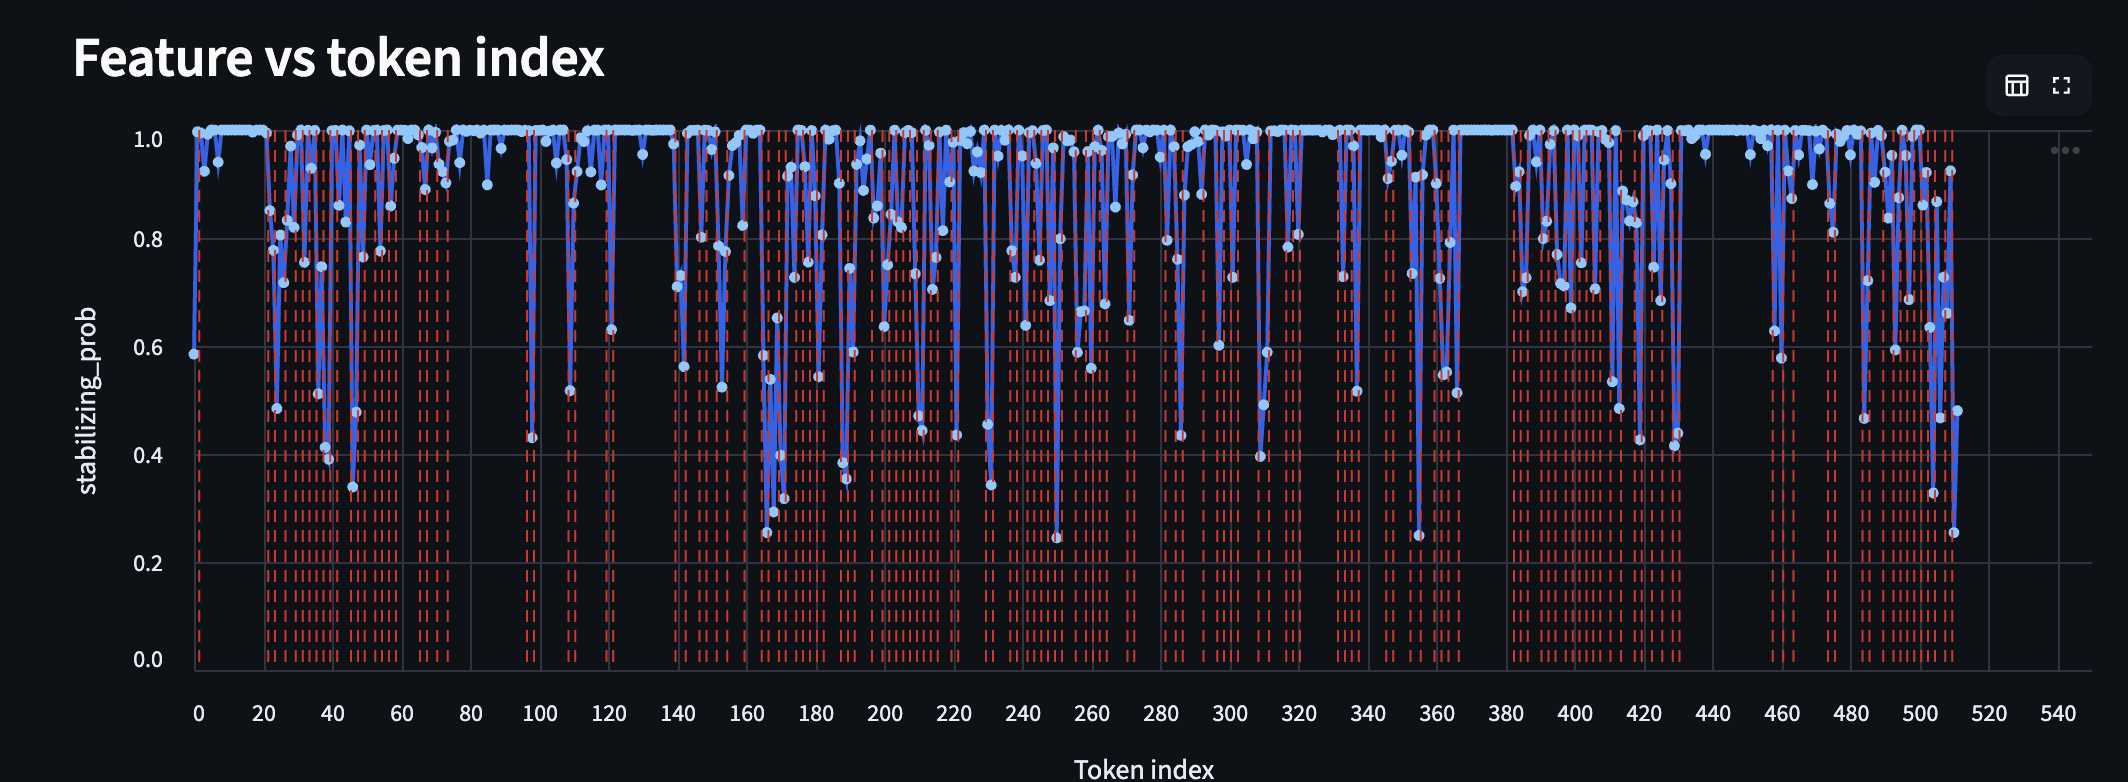
\includegraphics[width=\linewidth]{../phase_cpd/results_pelt/pelt_images/algebra_images/algebra_stab_prob.png}
    \caption{Algebra: raw stabilizing probability.}
  \end{subfigure}
  \hfill
  \begin{subfigure}{0.30\linewidth}
    \centering
    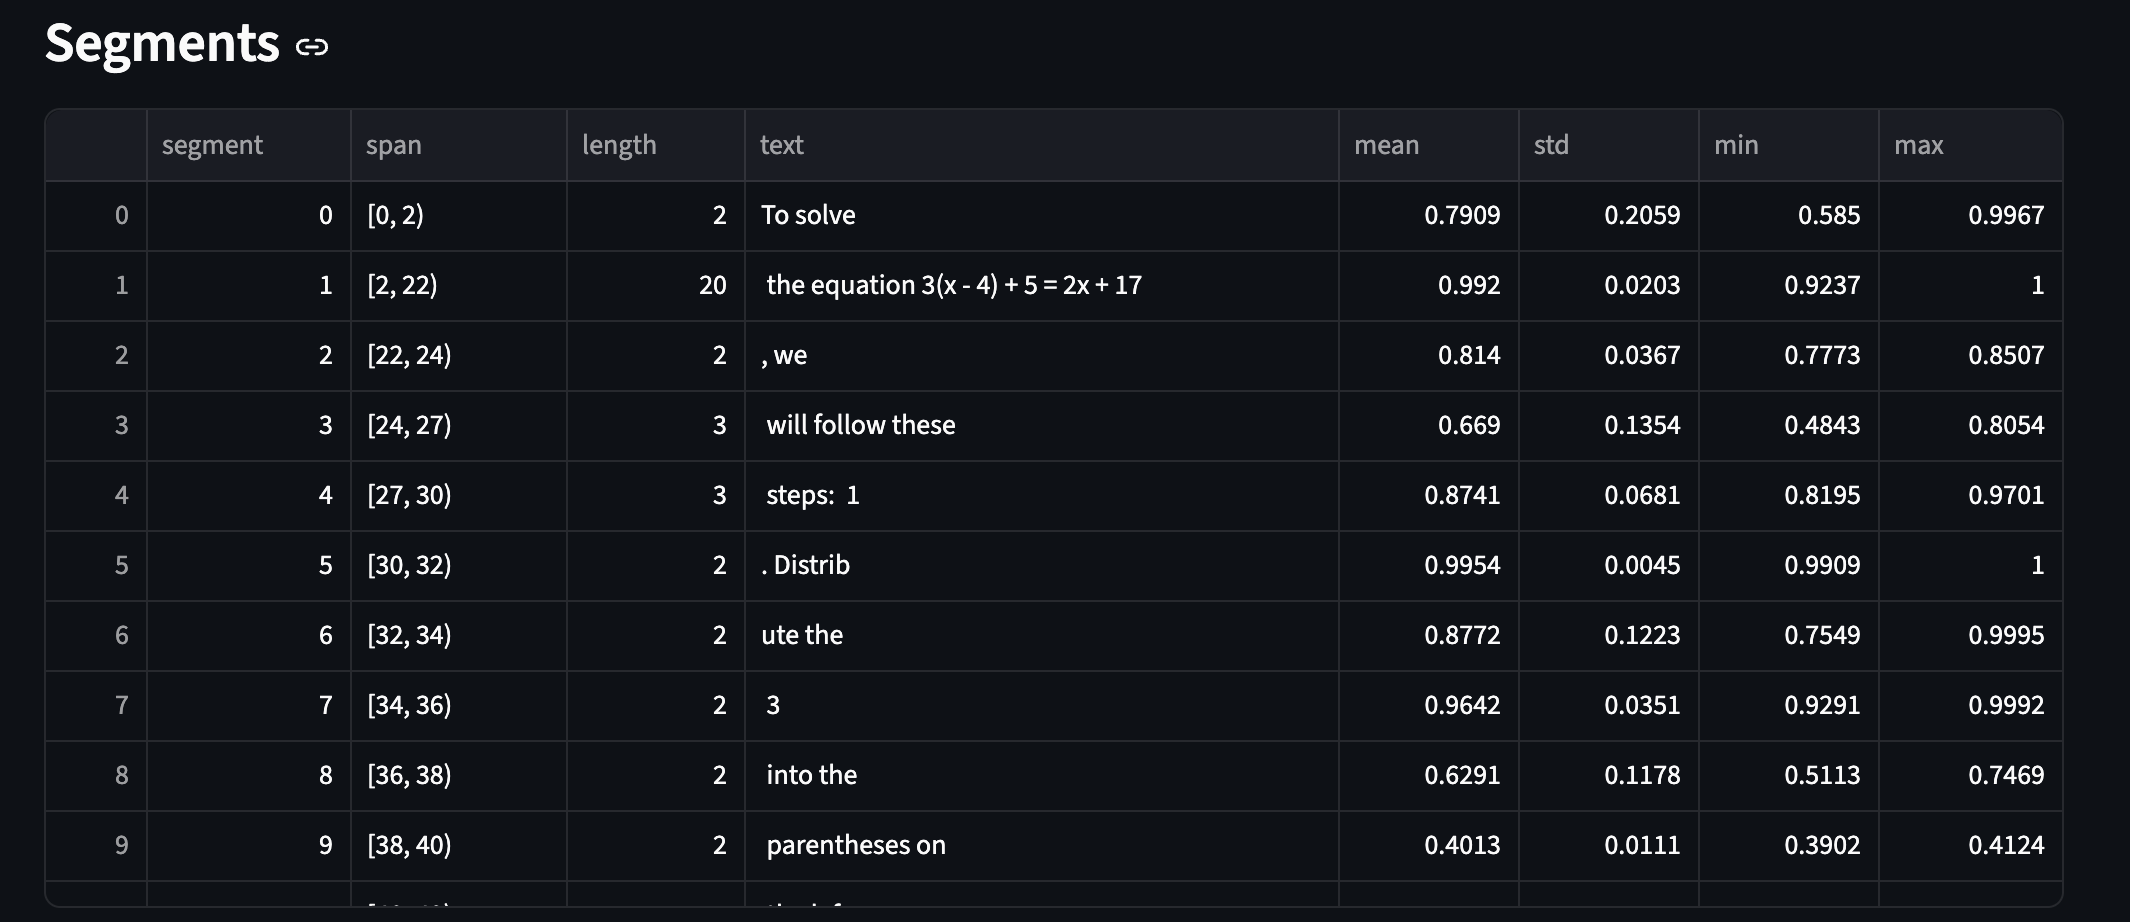
\includegraphics[width=\linewidth]{../phase_cpd/results_pelt/pelt_images/algebra_images/algebra_stab_prob_segments.png}
    \caption{Algebra: probability with PELT segments.}
  \end{subfigure}
  \hfill
  \begin{subfigure}{0.30\linewidth}
    \centering
    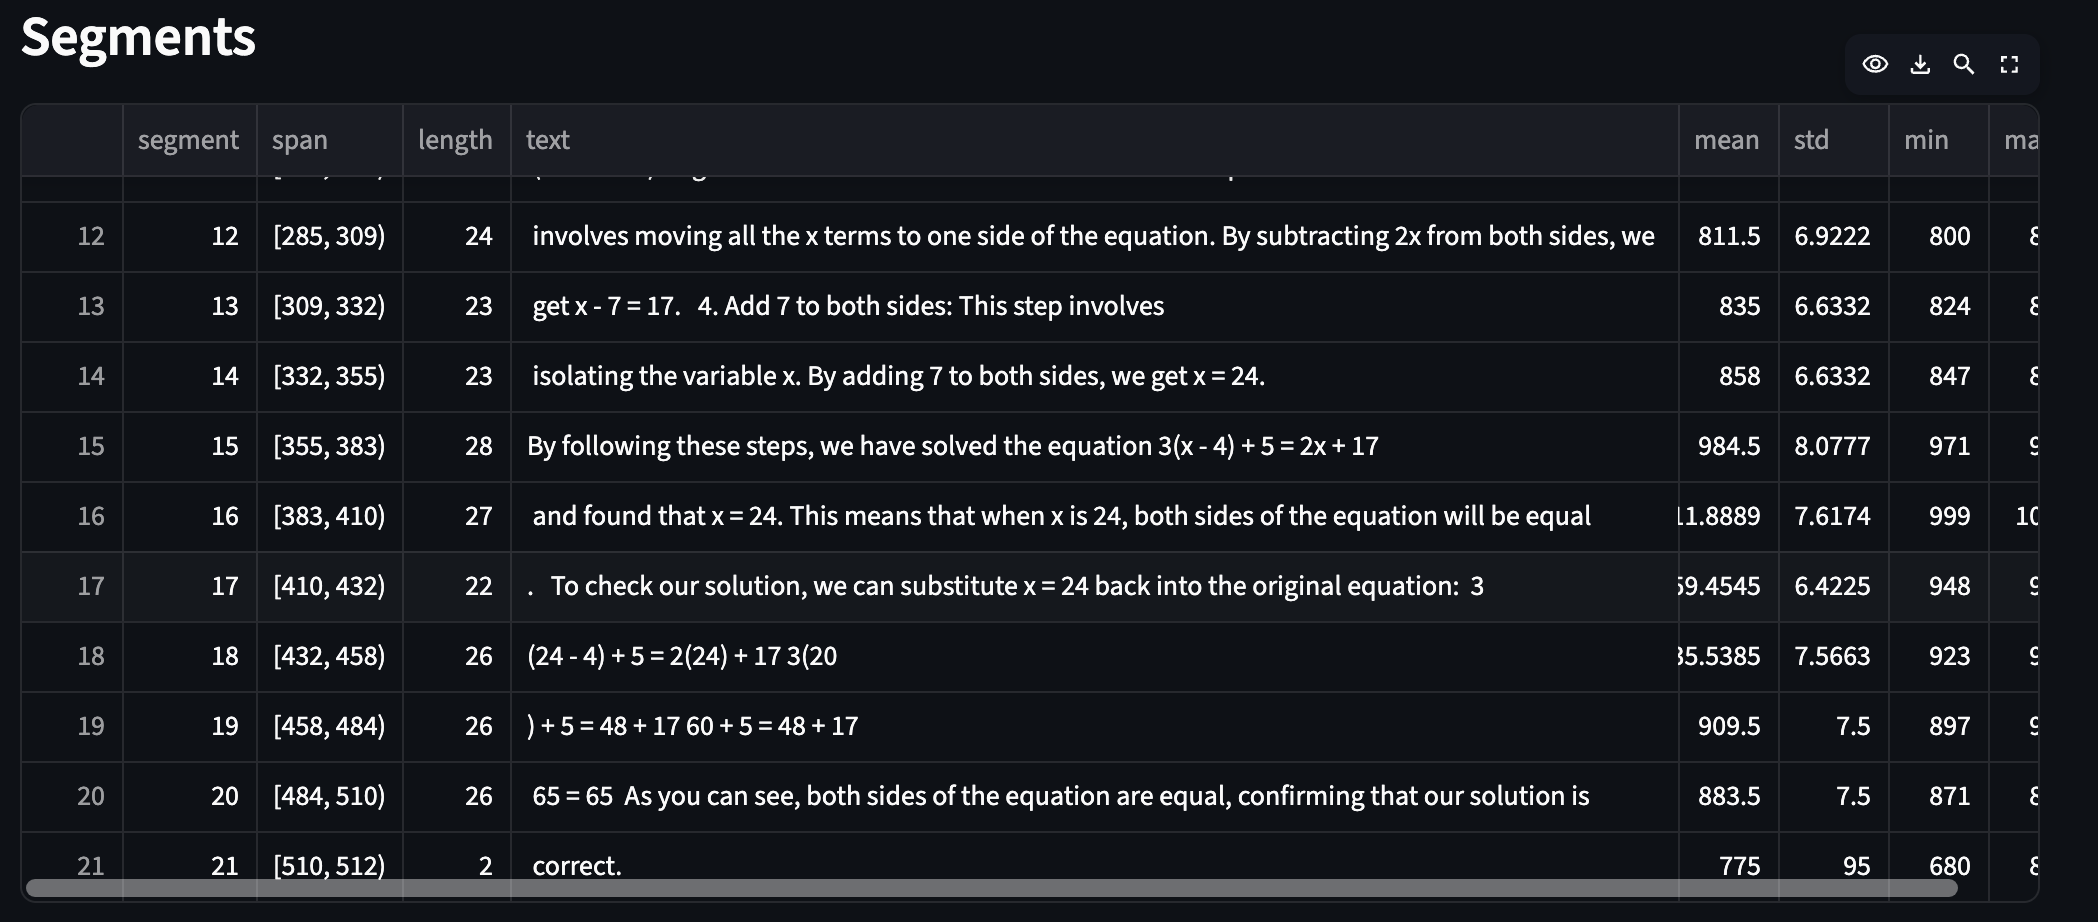
\includegraphics[width=\linewidth]{../phase_cpd/results_pelt/pelt_images/algebra_images/algebra_stab_ref_steps_segments.png}
    \caption{Algebra: refinement-step signal.}
  \end{subfigure}

  \vspace{0.22cm}
  \begin{subfigure}{0.30\linewidth}
    \centering
    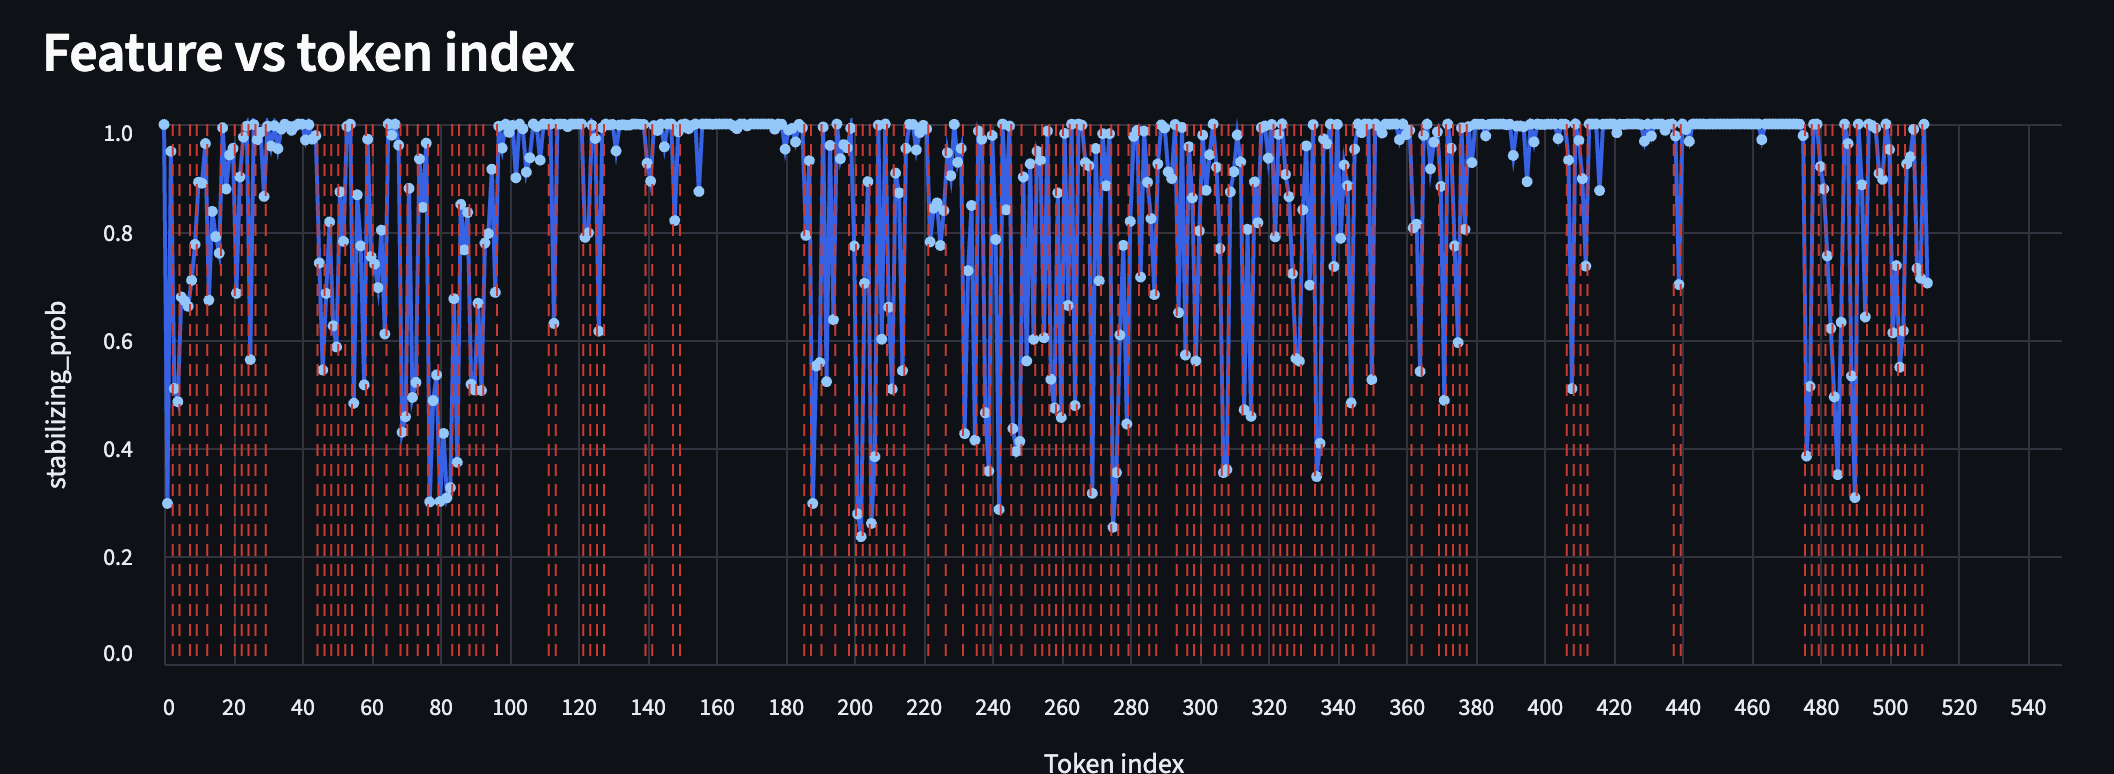
\includegraphics[width=\linewidth]{../phase_cpd/results_pelt/pelt_images/binary_search_images/binary_stab_prob.png}
    \caption{Binary search: raw stabilizing probability.}
  \end{subfigure}
  \hfill
  \begin{subfigure}{0.30\linewidth}
    \centering
    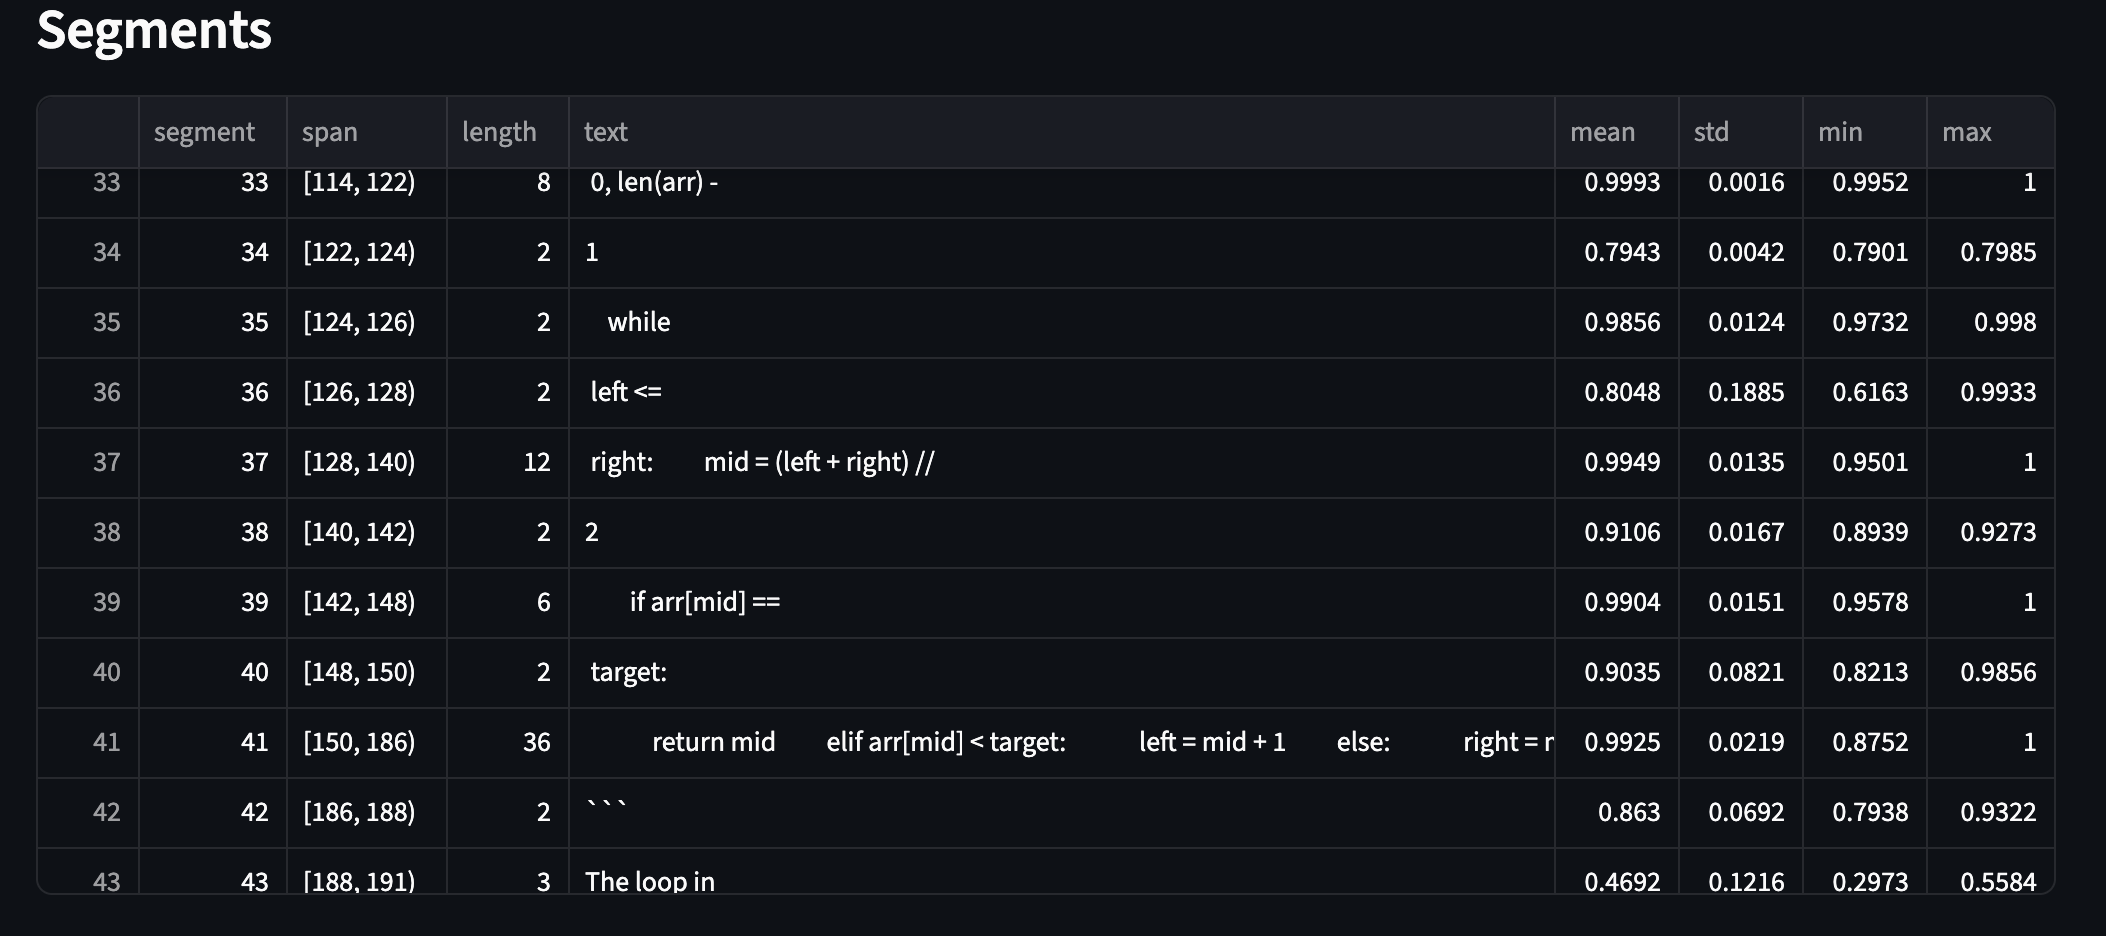
\includegraphics[width=\linewidth]{../phase_cpd/results_pelt/pelt_images/binary_search_images/binary_stab_prob_segments.png}
    \caption{Binary search: probability with PELT segments.}
  \end{subfigure}
  \hfill
  \begin{subfigure}{0.30\linewidth}
    \centering
    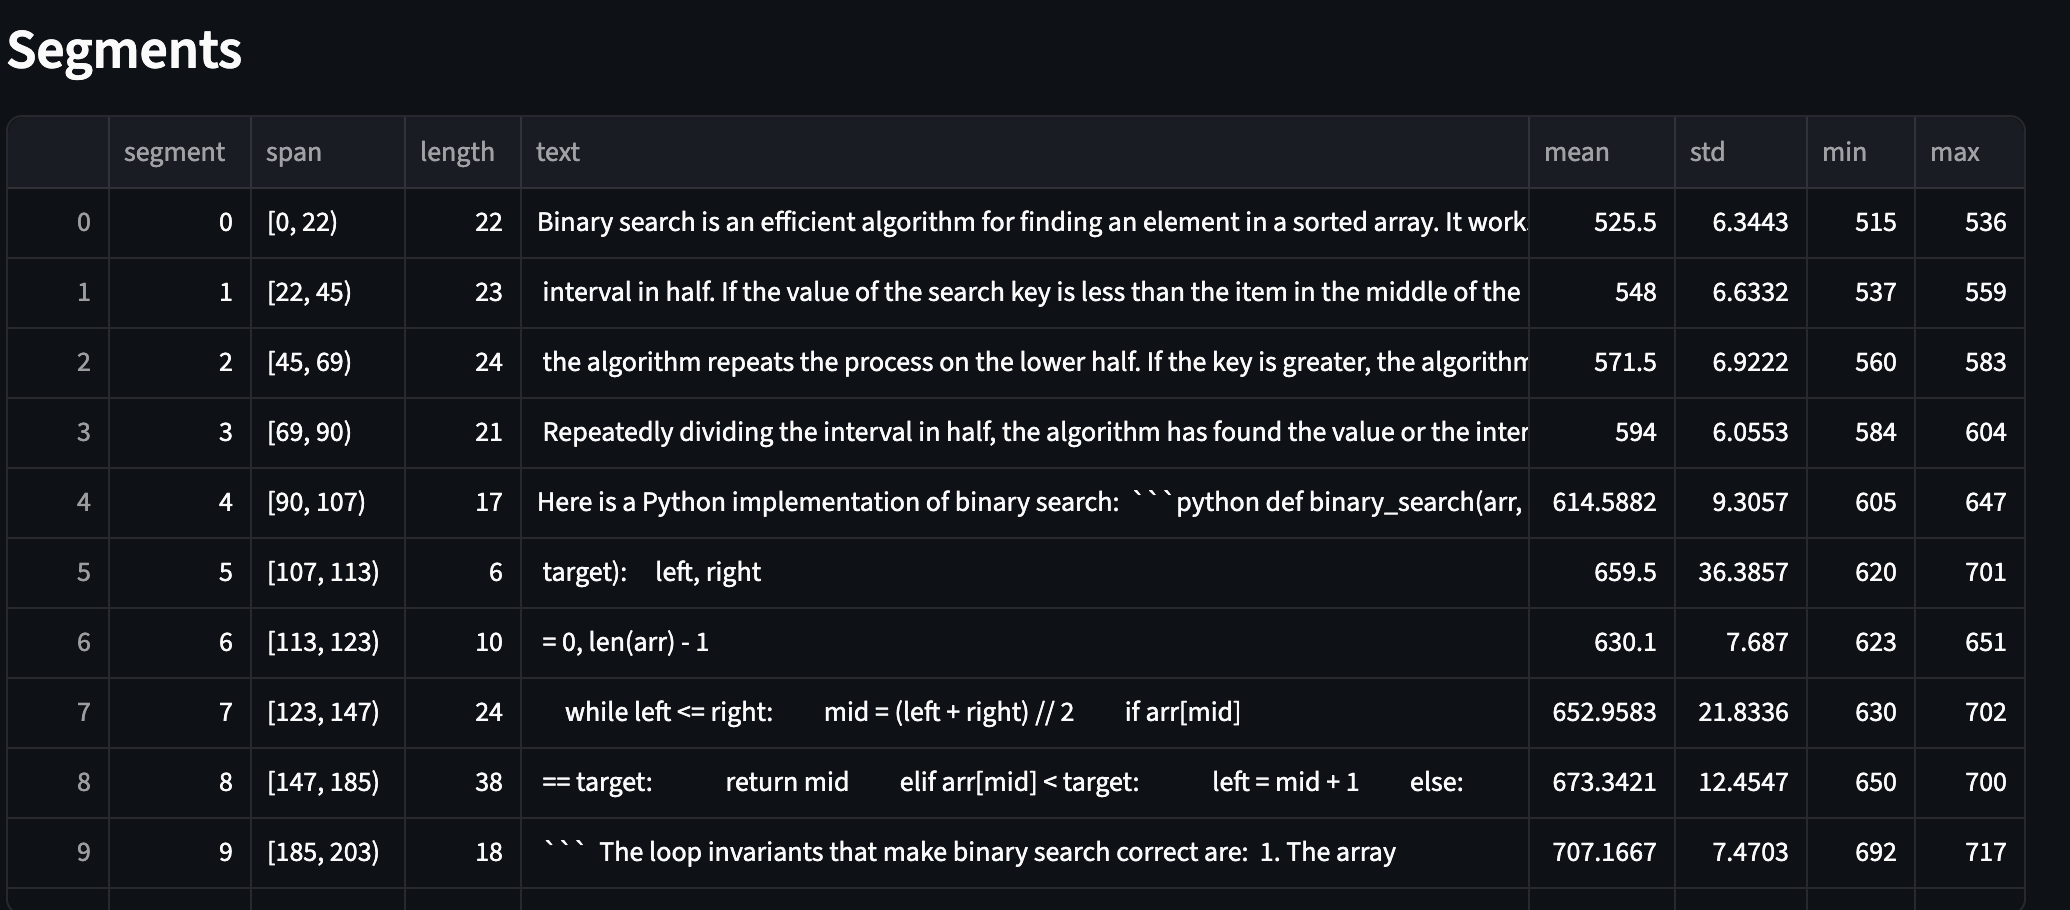
\includegraphics[width=\linewidth]{../phase_cpd/results_pelt/pelt_images/binary_search_images/binary_stab_ref_steps_segments.png}
    \caption{Binary search: refinement-step signal.}
  \end{subfigure}
  \caption{Token-level CPD analysis for two representative prompts (algebra and binary search). Left column: raw stabilizing probability curves showing high-confidence plateaus alternating with low-confidence computation spans. Center column: same curves overlaid with PELT-detected segment boundaries. Right column: stabilizing refinement step, which is more monotonic across token position.}
  \label{fig:cpd}
\end{figure}

\subsection{Block-Native AdaBlock Traces}

The final training path uses AdaBlock-style LLaDA traces. We ran LLaDA-8B-Instruct on GSM8K and recorded one tuple per decoded block. Each tuple contains the applied block size, actual \nfe{}, token stabilization/refinement summaries, top-1 confidence statistics, digit fraction, delimiter fraction, and gap statistics. The training corpus contains 5{,}000 GSM8K training problems with 138{,}901 blocks and 200 validation/test problems with 5{,}543 blocks. A separate 200-prompt test slice (GSM8K test indices 200--399) is used for downstream scheduler evaluation.

\begin{figure}[!htbp]
  \centering
  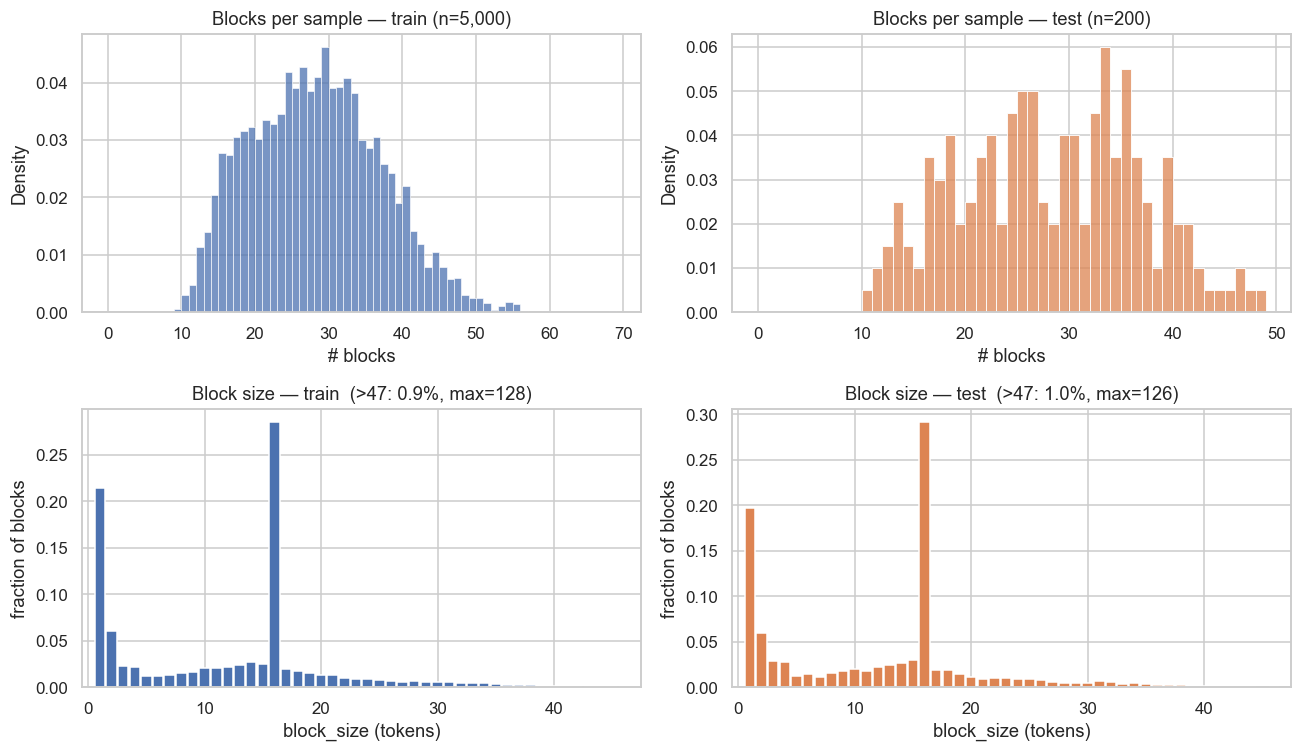
\includegraphics[width=0.88\linewidth]{figs/block_structure.png}
  \caption{AdaBlock block structure on GSM8K. Blocks per sample are similar between train and test, while block sizes have strong point masses at size 1 and 16.}
  \label{fig:block-structure}
\end{figure}

Figure~\ref{fig:block-structure} shows why the prediction problem is not a smooth regression problem. The schedule has a heavy point mass at delimiter-size blocks and a large mass at the content cap. A predictor that averages targets can be numerically close under MSE while producing poor discrete controls.

\begin{figure}[!htbp]
  \centering
  \begin{tabular}{@{}ccc@{}}
    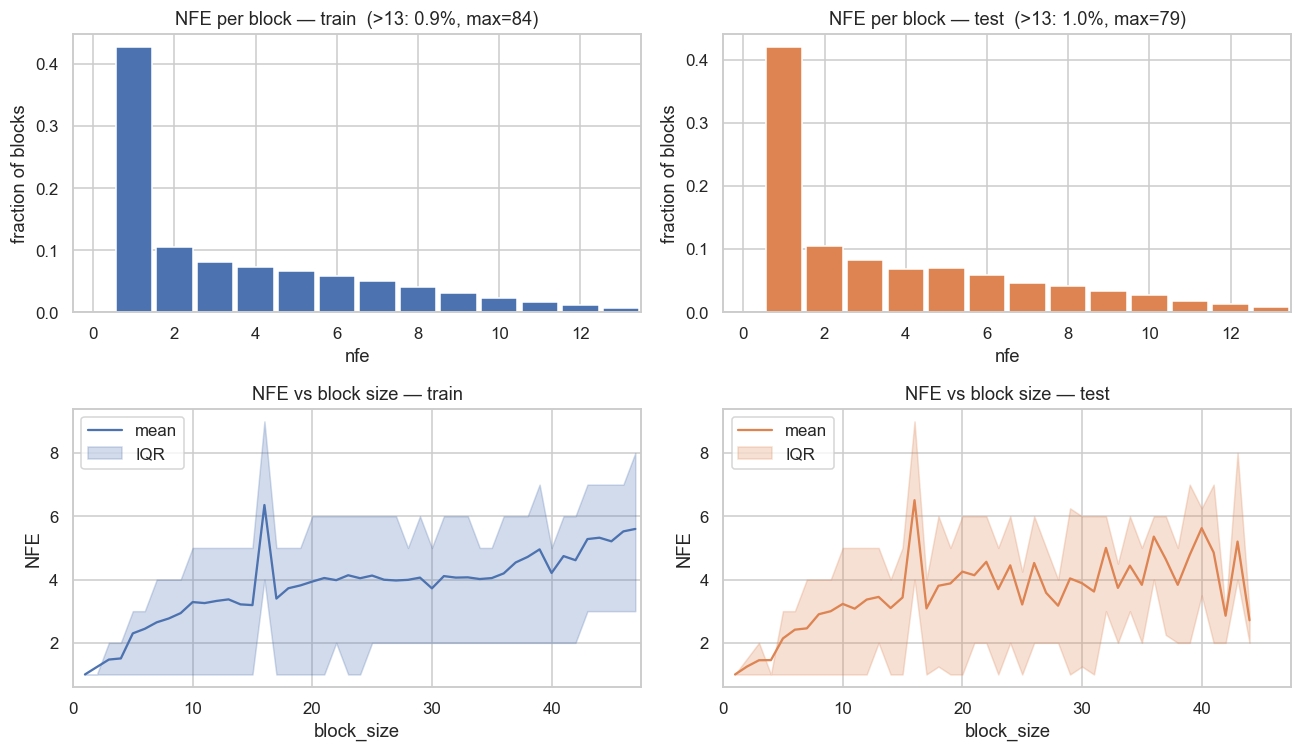
\includegraphics[width=0.31\linewidth, trim=0 376 651 0, clip]{figs/nfe.png} &
    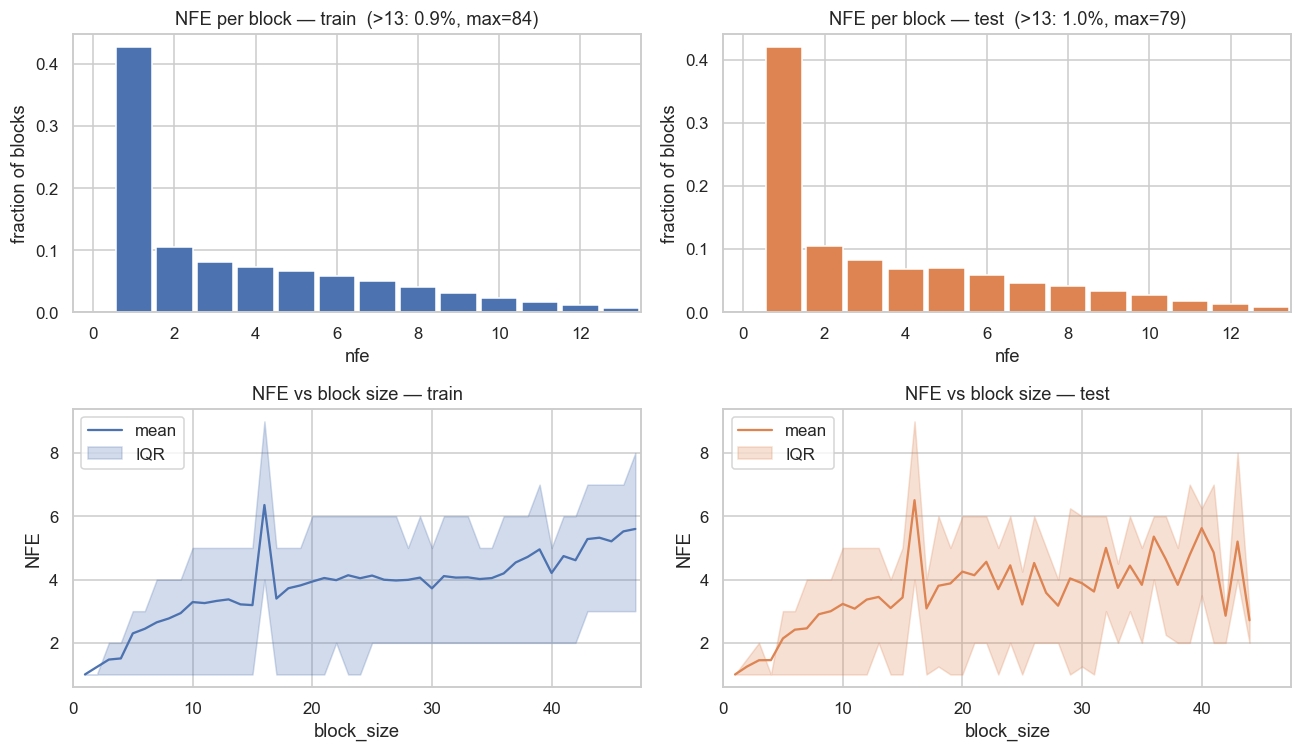
\includegraphics[width=0.31\linewidth, trim=651 376 0 0, clip]{figs/nfe.png} &
    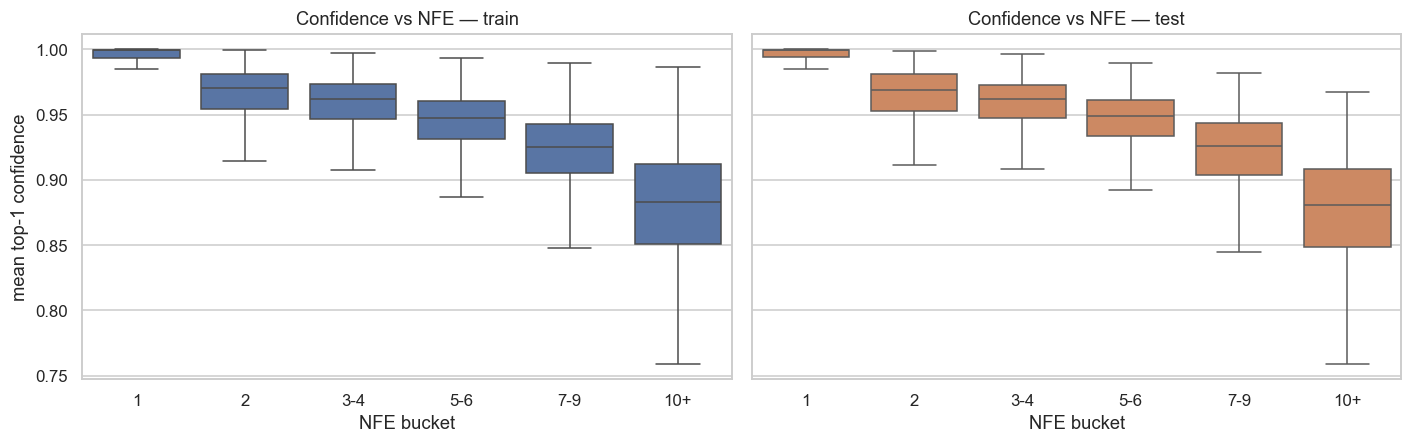
\includegraphics[width=0.31\linewidth, trim=0 0 706 0, clip]{figs/confidence_vs_nfe.png} \\[-0.15em]
    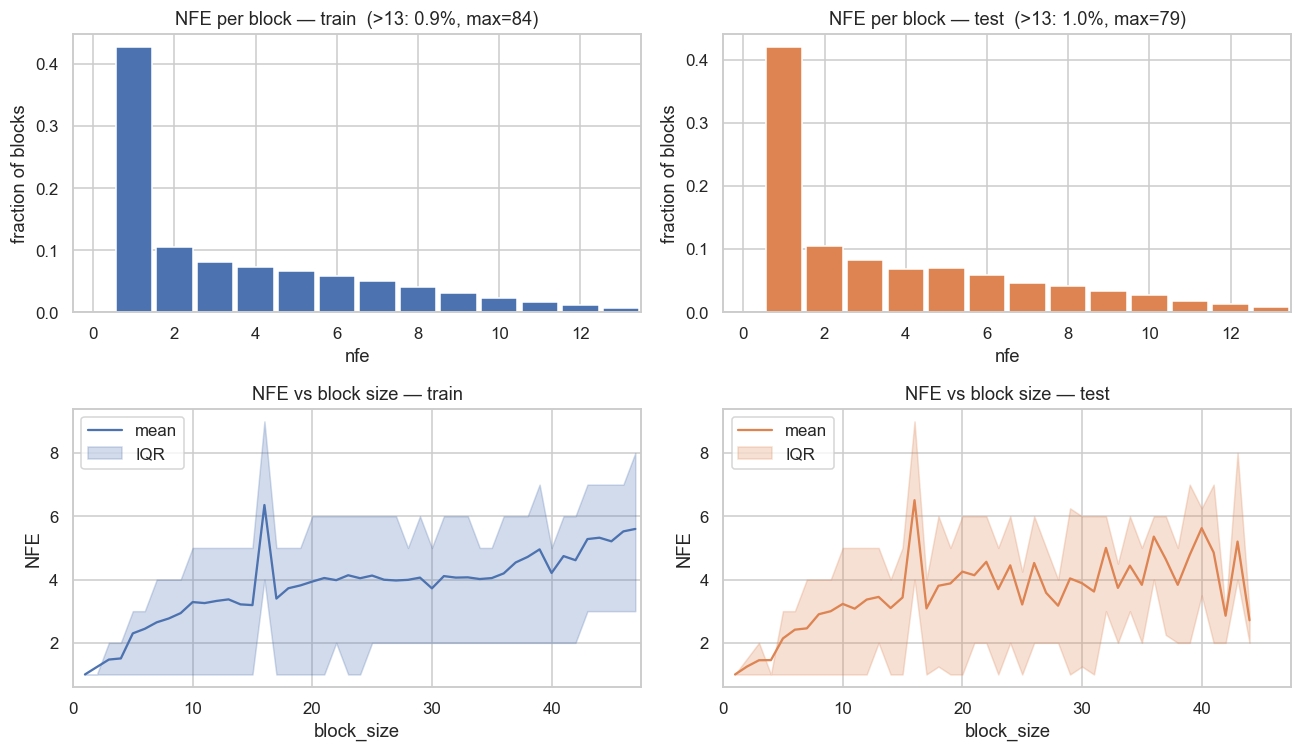
\includegraphics[width=0.31\linewidth, trim=0 0 651 376, clip]{figs/nfe.png} &
    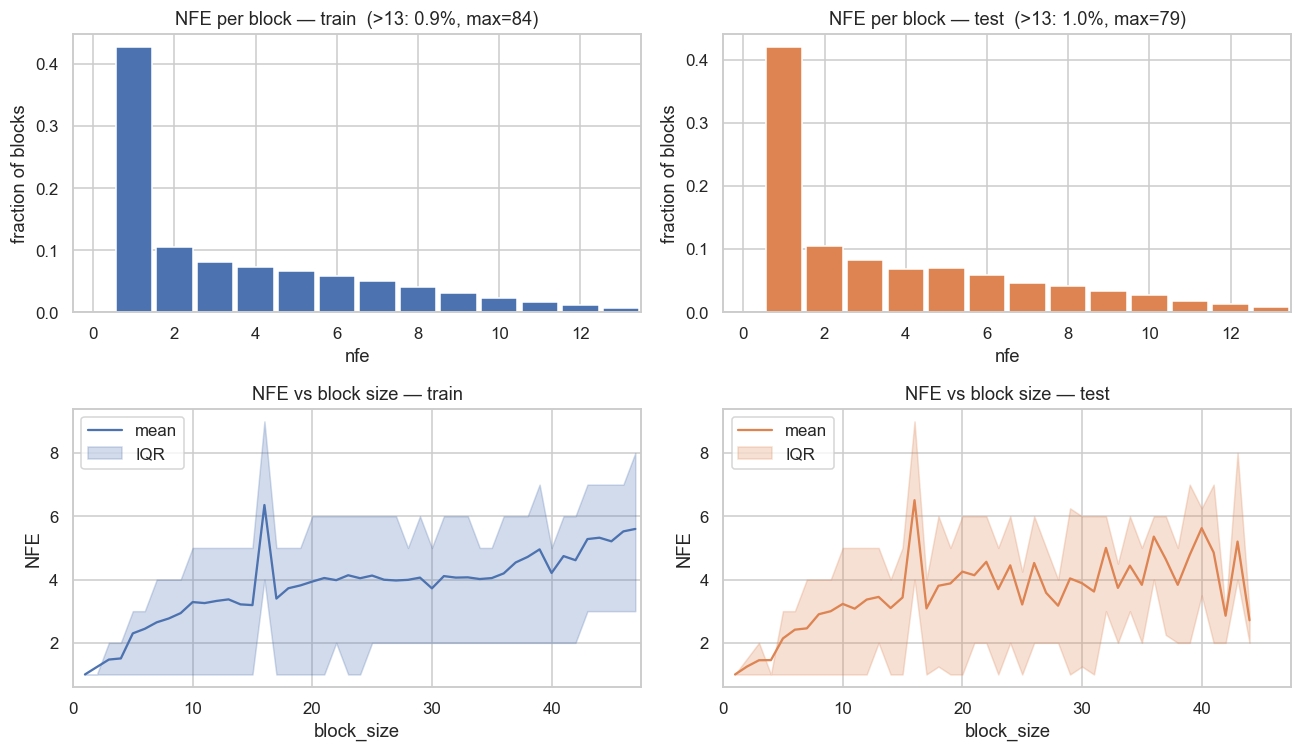
\includegraphics[width=0.31\linewidth, trim=651 0 0 376, clip]{figs/nfe.png} &
    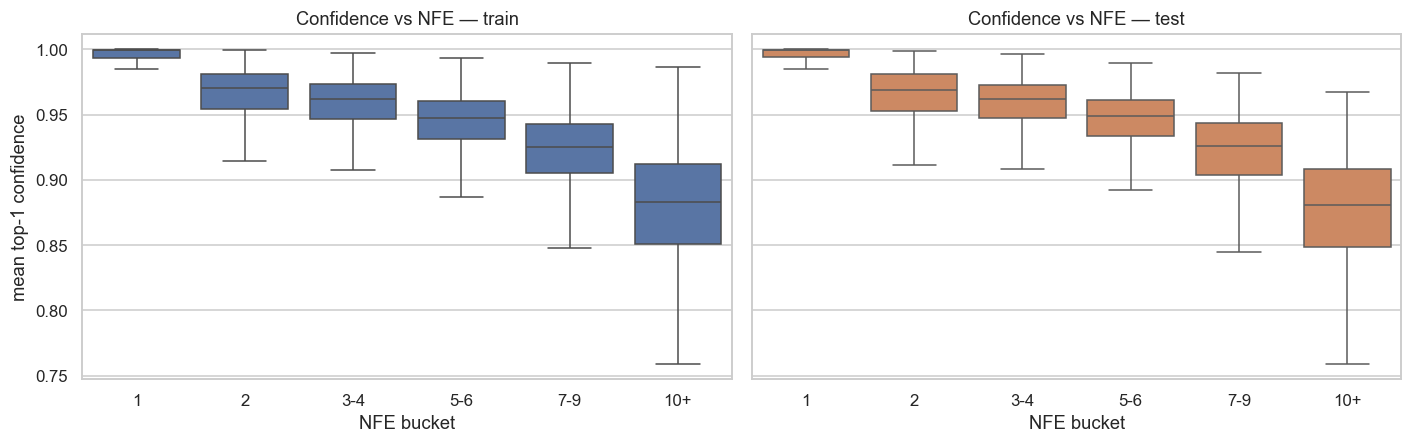
\includegraphics[width=0.31\linewidth, trim=760 0 0 0, clip]{figs/confidence_vs_nfe.png}
  \end{tabular}
  \caption{Per-block compute and confidence. \nfe{} grows with block size but has wide conditional variance, while high-compute blocks are lower-confidence and more variable.}
  \label{fig:nfe}
  \label{fig:conf-vs-nfe}
\end{figure}

\section{Predictors}

\subsection{Regression Transformer}

The first learned predictor treated the next tuple as a continuous regression target. A compact Transformer encoder consumed a sliding window of previous tuples, projected them to a hidden dimension, added sinusoidal position encodings, pooled the final context position, and produced real-valued outputs. Inference rounded outputs back to integer controls. This model was easy to extend from two features to rich tuples, and several checkpoints reached validation losses near \(0.096\) on normalized tuple targets. The failure mode was deployment-oriented: MSE encouraged averaged predictions in a discrete, multimodal target space.

\subsection{Classification/Ordinal Transformer}

The final predictor keeps the Transformer encoder but changes the heads. The block-size head is a classifier over possible block sizes. The stabilization/\nfe{} head is ordinal: it predicts threshold logits and recovers the budget by counting thresholds whose sigmoid exceeds 0.5. The stabilization head is conditioned on block logits, so the model can represent that larger blocks often require different refinement budgets.

\begin{figure}[!htbp]
  \centering
  \resizebox{0.94\linewidth}{!}{%
  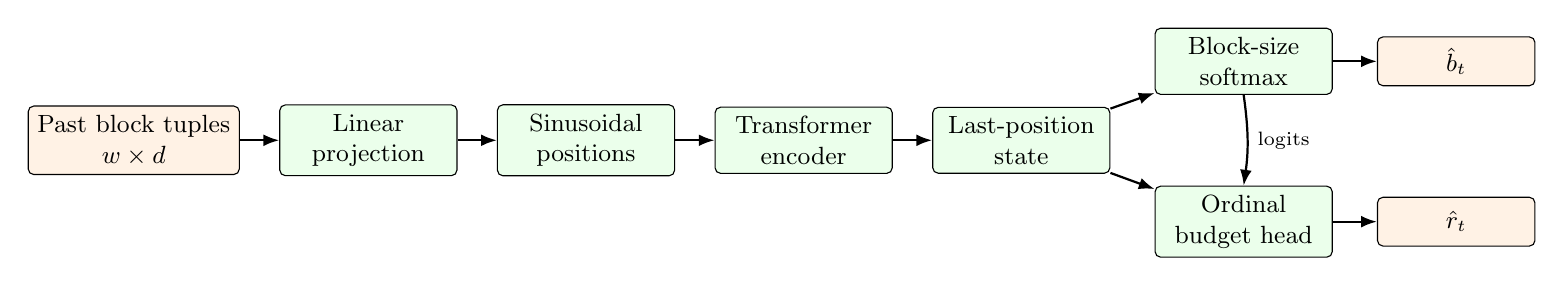
\begin{tikzpicture}[node distance=0.58cm and 0.5cm]
    \node[data] (inp) {Past block tuples\\\(w \times d\)};
    \node[modelbox, right=of inp] (proj) {Linear\\projection};
    \node[modelbox, right=of proj] (pos) {Sinusoidal\\positions};
    \node[modelbox, right=of pos] (enc) {Transformer\\encoder};
    \node[modelbox, right=of enc] (pool) {Last-position\\state};
    \node[modelbox, above right=0.15cm and 0.56cm of pool] (block) {Block-size\\softmax};
    \node[modelbox, below right=0.15cm and 0.56cm of pool] (stab) {Ordinal\\budget head};
    \node[data, right=0.56cm of block] (bout) {\(\hat b_t\)};
    \node[data, right=0.56cm of stab] (sout) {\(\hat r_t\)};
    \draw[arrow] (inp) -- (proj);
    \draw[arrow] (proj) -- (pos);
    \draw[arrow] (pos) -- (enc);
    \draw[arrow] (enc) -- (pool);
    \draw[arrow] (pool) -- (block);
    \draw[arrow] (pool) -- (stab);
    \draw[arrow] (block) -- (bout);
    \draw[arrow] (stab) -- (sout);
    \draw[arrow] (block.south) to[bend left=8] node[midway, right, font=\scriptsize]{logits} (stab.north);
  \end{tikzpicture}
  }
  \caption{Classification/ordinal Transformer architecture. The block-size logits condition the refinement-budget head.}
  \label{fig:model-arch}
\end{figure}

Training uses cross-entropy for block size and binary cross-entropy for ordinal budget thresholds. The implementation supports a 6-feature and 12-feature input mode. The final scheduler checkpoint used the rich-feature classifier path and was integrated through \code{AdaBlock-dLLM/llada/pag\_predictor.py}.

\subsection{Other Predictor Experiments}

We also explored two non-Transformer baselines.

\textbf{Variable-order Markov model.} The VOMM predictor memorizes recent tuple contexts and backs off when a context is unseen. It is useful as a sanity check because it is cheap and interpretable, but it cannot generalize well to continuous confidence features or unseen block patterns.

\textbf{Random forest.} The \code{rf-block-stab-predict} branch trained a multi-output random forest on rolling-window statistics. With window size 5, 200 trees, max depth 15, and features \(\{\) \nfe{}, block size, max stabilization step, mean refinement step, mean gap, max gap \(\}\), it trained on 90{,}994 examples and tested on 22{,}907 examples. Its held-out MAE was 7.24 for block size and 1.66 for max stabilization step. Figure~\ref{fig:rf-ablation} shows that the most predictive feature was the last observed block size, followed by window variability and trend features. This baseline supported the decision to keep history statistics in the learned setting, but the Transformer remained better matched to sequential deployment.

\begin{figure}[!htbp]
  \centering
  \begin{subfigure}{0.47\linewidth}
    \centering
    \begin{tikzpicture}
      \begin{axis}[
        xbar, width=\linewidth, height=5.5cm,
        xmin=0, xlabel={importance},
        symbolic y coords={block\_size\_last,block\_size\_std,block\_size\_trend,mean\_ref\_step\_trend,mean\_gap\_std,mean\_gap\_trend,mean\_ref\_step\_mean,mean\_ref\_step\_std,mean\_gap\_mean,mean\_ref\_step\_last},
        ytick=data, yticklabel style={font=\scriptsize},
        xticklabel style={font=\scriptsize},
      ]
        \addplot[fill=blue!35] table[x=importance,y=feature] {figs/rf_importance.tsv};
      \end{axis}
    \end{tikzpicture}
    \caption{Random forest feature importance.}
  \end{subfigure}
  \hfill
  \begin{subfigure}{0.49\linewidth}
    \centering
    \begin{tikzpicture}
      \begin{axis}[
        ybar, width=\linewidth, height=5.5cm,
        ylabel={best validation loss},
        xtick=data, xticklabels from table={figs/ablation_bestvals.tsv}{run},
        x tick label style={rotate=45, anchor=east, font=\tiny},
        yticklabel style={font=\scriptsize},
        ymin=0, bar width=7pt,
      ]
        \addplot[fill=green!35] table[x expr=\coordindex,y=val_loss] {figs/ablation_bestvals.tsv};
      \end{axis}
    \end{tikzpicture}
    \caption{Best saved Transformer ablation checkpoints.}
  \end{subfigure}
  \caption{Predictor experiments beyond the final scheduler. The RF branch provided interpretable feature rankings; Transformer ablations tested context length, hidden size, heads, layers, dropout, and learning rate.}
  \label{fig:rf-ablation}
\end{figure}

\section{Tuple-Conditioned Scheduling}

The final scheduler integrates the predictor into LLaDA generation. For each block, it builds a padded history of realized block outcomes, predicts the next control tuple, clips it by remaining length and configured bounds, and runs LLaDA refinement on that active span. The implementation records the realized block size, actual \nfe{}, confidence statistics, digit fraction, and delimiter fraction, then appends that tuple to the history before the next prediction.

Several engineering changes were necessary to make the learned scheduler comparable to AdaBlock:
\begin{itemize}[leftmargin=1.3em, itemsep=0.1em]
  \item \textbf{Seed alignment.} The final comparator seeds PAG from AdaBlock's realized first block for the same prompt. This removes an artifact where separate probes created unfair first-block differences.
  \item \textbf{Reactive safeguards.} The branch \code{feat/reactive-block-predictive-budget} added reactive block sizing, predictive residual budgeting, soft exit gates, and a fix preventing the ``few remaining'' gate from force-committing low-confidence tokens.
  \item \textbf{Caching.} Prefix-cache and dual-cache variants preserve tuple-conditioned scheduling while reducing repeated computation in LLaDA.
  \item \textbf{Visualization.} The log viewers flatten prompt, method, delta, and block histories into dashboards for qualitative inspection.
\end{itemize}

\begin{figure}[!htbp]
  \centering
  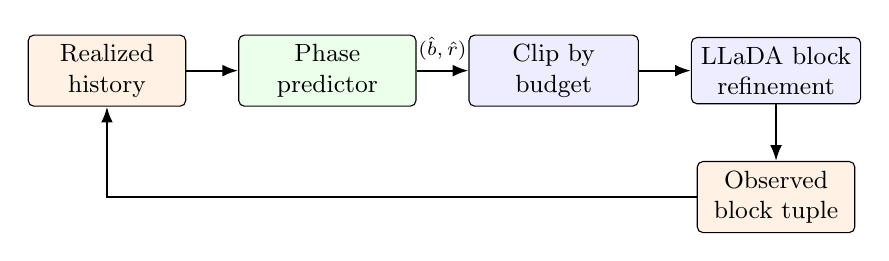
\begin{tikzpicture}[node distance=0.62cm and 0.66cm]
    \node[data] (hist) {Realized\\history};
    \node[modelbox, right=of hist] (pred) {Phase\\predictor};
    \node[stage, right=of pred] (clip) {Clip by\\budget};
    \node[stage, right=of clip] (llada) {LLaDA block\\refinement};
    \node[data, below=0.72cm of llada] (obs) {Observed\\block tuple};
    \draw[arrow] (hist) -- (pred);
    \draw[arrow] (pred) -- node[above, font=\scriptsize]{\((\hat b,\hat r)\)} (clip);
    \draw[arrow] (clip) -- (llada);
    \draw[arrow] (llada) -- (obs);
    \draw[arrow] (obs.west) -| (hist.south);
  \end{tikzpicture}
  \caption{Deployment loop. Predictions are not only offline labels: they directly control the next LLaDA block and are updated with realized outcomes.}
  \label{fig:scheduler-loop}
\end{figure}

\section{Evaluation}

\subsection{Setup}

We evaluate on 200 GSM8K test prompts, \code{gsm8k\_test\_0200}--\code{gsm8k\_test\_0399}, using LLaDA-8B-Instruct with generation length 256, 64 diffusion steps, confidence threshold 0.9, delimiter threshold 0.3, prefix+dual cache, minimum block length 1, minimum refinement budget 1, and no refinement offset. The final log file contains multiple runs; the reported numbers use the latest complete 200-prompt run, \code{\FinalRunId}. The answer metric is exact presence of the accepted numeric answer in the generated text after normalization, matching the repository evaluator.

\begin{table}[!htbp]
  \centering
  \begin{tabular}{lrrrr}
    \toprule
    Method & Accuracy & Correct & Avg. total \nfe{} & Avg. blocks \\
    \midrule
    PAG & \PagAccPct\% & \PagCorrect/\FinalNumPrompts & \PagAvgNfe & \PagAvgBlocks \\
    AdaBlock & \AdaAccPct\% & \AdaCorrect/\FinalNumPrompts & \AdaAvgNfe & \AdaAvgBlocks \\
    \bottomrule
  \end{tabular}
  \caption{Final 200-prompt GSM8K evaluation. PAG matches AdaBlock answer accuracy while using fewer forward evaluations.}
  \label{tab:final-eval}
\end{table}

\begin{figure}[!htbp]
  \centering
	  \begin{subfigure}{0.46\linewidth}
	    \centering
	    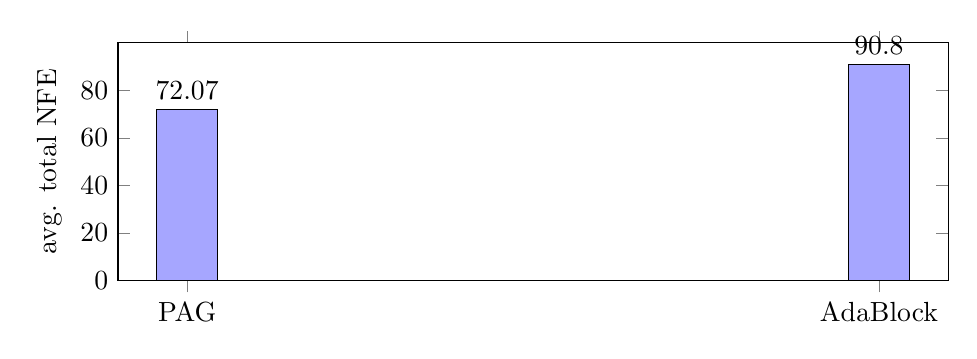
\begin{tikzpicture}
	      \begin{axis}[
	        ybar, width=\linewidth, height=4.6cm,
        ylabel={avg. total \nfe{}}, symbolic x coords={PAG,AdaBlock},
        xtick=data, ymin=0, bar width=22pt, nodes near coords,
      ]
        \addplot[fill=blue!35] coordinates {(PAG,\PagAvgNfe) (AdaBlock,\AdaAvgNfe)};
      \end{axis}
    \end{tikzpicture}
    \caption{Average compute.}
  \end{subfigure}
  \hfill
  \begin{subfigure}{0.46\linewidth}
    \centering
    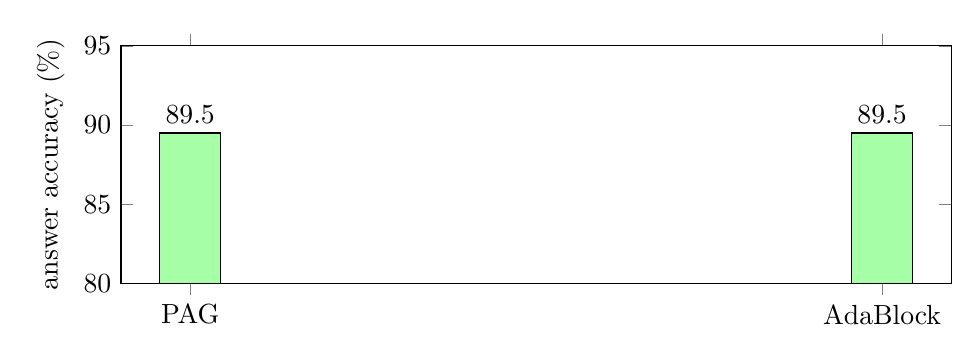
\begin{tikzpicture}
      \begin{axis}[
        ybar, width=\linewidth, height=4.6cm,
        ylabel={answer accuracy (\%)}, symbolic x coords={PAG,AdaBlock},
        xtick=data, ymin=80, ymax=95, bar width=22pt, nodes near coords,
      ]
        \addplot[fill=green!35] coordinates {(PAG,\PagAccPct) (AdaBlock,\AdaAccPct)};
      \end{axis}
	    \end{tikzpicture}
	    \caption{Answer accuracy.}
	  \end{subfigure}
	  \caption{Aggregate final evaluation. PAG matches AdaBlock answer accuracy while using fewer forward evaluations.}
	  \label{fig:final-eval-summary}
	\end{figure}

\begin{figure}[!htbp]
  \centering
	  \begin{subfigure}{0.46\linewidth}
	    \centering
	    \begin{tikzpicture}
	      \begin{axis}[
        ybar, width=\linewidth, height=4.6cm,
        xlabel={PAG - AdaBlock \nfe{} delta}, ylabel={prompts},
        xtick=data, xticklabels from table={figs/nfe_delta_hist.tsv}{bin},
        x tick label style={rotate=45, anchor=east, font=\tiny},
        ymin=0, bar width=6pt,
      ]
        \addplot[fill=orange!45] table[x expr=\coordindex,y=count] {figs/nfe_delta_hist.tsv};
      \end{axis}
    \end{tikzpicture}
    \caption{\nfe{} savings distribution.}
  \end{subfigure}
  \hfill
  \begin{subfigure}{0.46\linewidth}
    \centering
    \begin{tikzpicture}
      \begin{axis}[
        width=\linewidth, height=4.6cm,
        xlabel={AdaBlock total \nfe{}}, ylabel={PAG total \nfe{}},
        yticklabel style={font=\scriptsize}, xticklabel style={font=\scriptsize},
        legend style={font=\scriptsize, at={(0.03,0.97)}, anchor=north west},
      ]
        \addplot[only marks, mark=*, mark size=1.1pt, blue!65]
          table[x=adablock_nfe,y=pag_nfe] {figs/final_eval_points.tsv};
        \addplot[domain=35:170, dashed, black] {x};
        \legend{prompt, parity}
      \end{axis}
    \end{tikzpicture}
	    \caption{Per-prompt compute parity.}
	  \end{subfigure}
	  \caption{Per-prompt final evaluation plots. PAG reduced \nfe{} on \NfeWinCount{} of \FinalNumPrompts{} prompts, tied on \NfeTieCount{}, and used more \nfe{} on \NfeLossCount{}.}
	  \label{fig:final-eval}
\end{figure}

The average \nfe{} ratio was \(\AvgNfeRatio\), so PAG used about \(21.4\%\) fewer forward evaluations than AdaBlock. Median \nfe{} delta was \(\MedNfeDelta\), and average runtime delta was \(\AvgRuntimeDelta\) seconds. Runtime savings are smaller than \nfe{} savings because predictor calls and Python control overhead are visible at this evaluation scale, but the model compute component still decreased.

\begin{figure}[!htbp]
  \centering
  \begin{subfigure}{0.49\linewidth}
    \centering
    \begin{tikzpicture}
      \begin{axis}[
        width=\linewidth, height=4.8cm,
        xlabel={block index}, ylabel={value},
        legend style={font=\scriptsize},
        yticklabel style={font=\scriptsize}, xticklabel style={font=\scriptsize},
      ]
        \addplot[blue, mark=*] table[x=block,y=block_size] {figs/pag_saving_schedule.tsv};
        \addplot[orange, mark=square*] table[x=block,y=actual_nfe] {figs/pag_saving_schedule.tsv};
        \legend{block size, actual \nfe{}}
      \end{axis}
    \end{tikzpicture}
    \caption{\BestSavingPrompt{}: \BestSavingDelta{} \nfe{} delta.}
  \end{subfigure}
  \hfill
  \begin{subfigure}{0.49\linewidth}
    \centering
    \begin{tikzpicture}
      \begin{axis}[
        width=\linewidth, height=4.8cm,
        xlabel={block index}, ylabel={value},
        legend style={font=\scriptsize},
        yticklabel style={font=\scriptsize}, xticklabel style={font=\scriptsize},
      ]
        \addplot[blue, mark=*] table[x=block,y=block_size] {figs/pag_overhead_schedule.tsv};
        \addplot[orange, mark=square*] table[x=block,y=actual_nfe] {figs/pag_overhead_schedule.tsv};
        \legend{block size, actual \nfe{}}
      \end{axis}
    \end{tikzpicture}
    \caption{\WorstOverheadPrompt{}: +\WorstOverheadDelta{} \nfe{} delta.}
  \end{subfigure}
  \caption{Example PAG schedules from the final run. Most prompts save compute; the rare overhead cases occur when the learned schedule spends extra refinement on difficult blocks.}
  \label{fig:schedules}
\end{figure}

\FloatBarrier

\section{Discussion}

\textbf{What worked.} The strongest empirical result is that learned tuple scheduling can preserve AdaBlock-level GSM8K answer accuracy while reducing compute. The result is not just an offline predictor metric: it holds inside the LLaDA decoding loop, with predicted tuples controlling actual unmasking. The trace analysis also produced a useful interpretability story: confidence and stabilization dynamics line up with intuitive easy and hard regions.

\textbf{What did not fully work.} Regression losses were misleading because the scheduler controls are discrete and multimodal. CPD also became less central than originally planned; it was valuable for understanding traces, but too sensitive for permanent label construction. The random forest baseline was interpretable but less natural for rollout because it depends on hand-designed rolling statistics and does not model sequence context as directly.

\textbf{Why the final gains are plausible.} AdaBlock reacts to current confidence. PAG inherits an AdaBlock-compatible seed and then uses learned history to choose later blocks and budgets. The final run shows that many prompts need systematically less refinement than AdaBlock allocates, while accuracy disagreements are rare: PAG loses 2 prompts that AdaBlock solves and gains 2 prompts that AdaBlock misses across the complete final run.

\section{Limitations}

Our answer metric is a normalized numeric substring check, so it can miss reasoning quality differences that do not change the final answer. We evaluate one model family, LLaDA-8B-Instruct, and one benchmark slice, GSM8K test[200:400]. HumanEval, MBPP, MATH, and Dream integration remain natural follow-up evaluations. Runtime results should also be interpreted carefully: Python-side scheduler overhead is not optimized, and a fused implementation could change the wall-clock tradeoff.

The predictor is trained from AdaBlock traces, so it learns to imitate and improve around AdaBlock's operating regime rather than discovering schedules from first principles. Finally, we do not yet have a full learned model for future confidence/digit/delimiter features under rollout; during real decoding those features are observed after each block, but offline cost-aware evaluation must partially teacher-force non-control fields.

\section{Conclusion}

\pag{} frames adaptive \dllm{} decoding as a next-control prediction problem. Across the project, we built trace collection, CPD analysis, block-native tuple datasets, multiple predictor families, LLaDA scheduler integration, visualization dashboards, and a 200-prompt final evaluation. The most important design lesson is that phase structure is real but should be attached to the scheduler's native control space. On the final held-out GSM8K run, the learned scheduler matched AdaBlock answer accuracy while reducing average \nfe{} by about \(21\%\), showing that lightweight history-conditioned control is a viable direction for diffusion LLM reasoning systems.

\bibliographystyle{plainnat}
\small
\begin{thebibliography}{9}
\setlength{\itemsep}{0.05em}

\bibitem[Arriola et al.(2025)]{arriola2025block}
M.~Arriola, A.~Gokaslan, J.~T.~Chiu, Z.~Yang, Z.~Qi, J.~Han, S.~S.~Sahoo, and V.~Kuleshov.
\newblock Block diffusion: Interpolating between autoregressive and diffusion language models.
\newblock \emph{ICLR (Oral)}, 2025.

\bibitem[Gong et al.(2025)]{gong2025diffullama}
S.~Gong, S.~Agarwal, Y.~Zhang, J.~Ye, L.~Zheng, M.~Li, C.~An, P.~Zhao, W.~Bi, J.~Han, H.~Peng, and L.~Kong.
\newblock Scaling diffusion language models via adaptation from autoregressive models.
\newblock \emph{ICLR}, 2025.

\bibitem[Killick et al.(2012)]{killick2012optimal}
R.~Killick, P.~Fearnhead, and I.~A. Eckley.
\newblock Optimal detection of changepoints with a linear computational cost.
\newblock \emph{Journal of the American Statistical Association}, 107(500):1590--1598, 2012.

\bibitem[Lu et al.(2026)]{lu2025adablock}
G.~Lu, H.~M.~Chen, Y.~Karashima, Z.~Wang, D.~Fujiki, and H.~Fan.
\newblock AdaBlock-dLLM: Semantic-aware diffusion LLM inference via adaptive block size.
\newblock \emph{ICLR}, 2026.

\bibitem[Nie et al.(2025)]{nie2025llada}
S.~Nie, F.~Zhu, Z.~You, X.~Zhang, J.~Ou, J.~Hu, J.~Zhou, Y.~Lin, J.-R.~Wen, and C.~Li.
\newblock Large language diffusion models.
\newblock \emph{arXiv:2502.09992}, 2025.

\bibitem[Vaswani et al.(2017)]{vaswani2017attention}
A.~Vaswani, N.~Shazeer, N.~Parmar, J.~Uszkoreit, L.~Jones, A.~N. Gomez, L.~Kaiser, and I.~Polosukhin.
\newblock Attention is all you need.
\newblock \emph{NeurIPS}, 2017.

\bibitem[Wu et al.(2026)]{wu2025fastdllm}
C.~Wu, H.~Zhang, S.~Xue, Z.~Liu, S.~Diao, L.~Zhu, P.~Luo, S.~Han, and E.~Xie.
\newblock Fast-dLLM: Training-free acceleration of diffusion LLM by enabling KV cache and parallel decoding.
\newblock \emph{ICLR}, 2026.

\bibitem[Ye et al.(2025)]{ye2025dream}
J.~Ye, Z.~Xie, L.~Zheng, J.~Gao, Z.~Wu, X.~Jiang, Z.~Li, and L.~Kong.
\newblock Dream 7B: Diffusion large language models.
\newblock \emph{arXiv:2508.15487}, 2025.

\end{thebibliography}

\end{document}
